\documentclass[border=8pt]{standalone}
\usepackage{booktabs,array,xcolor,amsmath,graphicx}
\usepackage{tikz,pgfplots}
\pgfplotsset{compat=1.18}
\definecolor{ink}{RGB}{22,48,72}
\definecolor{accent}{RGB}{26,112,125}
\begin{document}
\begin{minipage}{15.2cm}\sffamily\small
{\Large\bfseries\color{ink} Recomputable ZVF on three retained reward tensors}\par\medskip
Qwen3-8B; GSM8K test; sampling only; $G=8$, $T=1.0$; 200 prompts per seed.\par\medskip
\begin{center}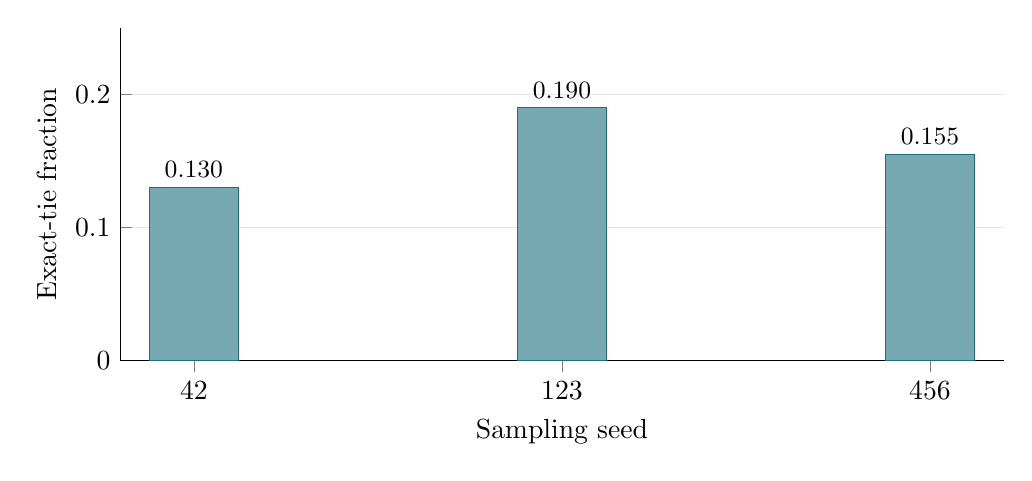
\begin{tikzpicture}
\begin{axis}[ybar,bar width=32pt,width=12.8cm,height=5.8cm,ymin=0,ymax=0.25,
 symbolic x coords={42,123,456},xtick=data,xlabel={Sampling seed},ylabel={Exact-tie fraction},
 nodes near coords,nodes near coords style={font=\small,/pgf/number format/fixed,/pgf/number format/precision=3,/pgf/number format/zerofill},axis lines*=left,ymajorgrids,grid style={gray!20}]
\addplot[fill=accent!60,draw=accent] coordinates {(42,0.130) (123,0.190) (456,0.155)};
\end{axis}\end{tikzpicture}\end{center}
Pooled count: $95/600=0.1583$. These are measured groups, not training gains. No synthetic variant ranking or imputed collapse classifier is shown.
\end{minipage}
\end{document}
